\documentclass[12pt]{article}
\usepackage{amsmath}
\usepackage{epsfig}
\usepackage{url}
%\usepackage{cite}
%\usepackage{array,multirow,dcolumn}
%\usepackage{rotate}


% This file is part of TUnfold.
%
% TUnfold is free software: you can redistribute it and/or modify
% it under the terms of the GNU General Public License as published by
% the Free Software Foundation, either version 3 of the License, or
% (at your option) any later version.
%
% TUnfold is distributed in the hope that it will be useful,
% but WITHOUT ANY WARRANTY; without even the implied warranty of
% MERCHANTABILITY or FITNESS FOR A PARTICULAR PURPOSE.  See the
% GNU General Public License for more details.
%
% You should have received a copy of the GNU General Public License
% along with TUnfold.  If not, see <http://www.gnu.org/licenses/>.

%\usepackage[]{lineno}
%\linenumbers
%%%%%%%%%%%%
\renewcommand{\topfraction}{1.0}
\renewcommand{\bottomfraction}{1.0}
\renewcommand{\textfraction}{0.0}
\newlength{\dinwidth}
\newlength{\dinmargin}
\setlength{\dinwidth}{21.0cm}
\textheight23.5cm \textwidth16.0cm
\setlength{\dinmargin}{\dinwidth}
\setlength{\unitlength}{1mm}
\addtolength{\dinmargin}{-\textwidth}
\setlength{\dinmargin}{0.5\dinmargin}
\oddsidemargin -1.0in
\addtolength{\oddsidemargin}{\dinmargin}
\setlength{\evensidemargin}{\oddsidemargin}
\setlength{\marginparwidth}{0.9\dinmargin}
\marginparsep 8pt \marginparpush 5pt
\topmargin -42pt
\headheight 12pt
\headsep 30pt \footskip 24pt
\parskip 3mm plus 2mm minus 2mm

\newcommand{\tunfoldmajor}{17}
\newcommand{\tunfoldminor}{3}
\newcommand{\tunfoldversion}{{\tunfoldmajor{}.\tunfoldminor}}

\newlength{\figwidth}
\setlength{\figwidth}{0.9\textwidth}

\newcommand{\mv}[1]{{\ensuremath{\boldsymbol{#1}}}}
\newcommand{\TR}[1]{\ensuremath{#1^{\sf T}}}
\newcommand{\mvTR}[1]{\TR{\mv{#1}}}
\begin{document}
\begin{titlepage}
\noindent
\begin{flushleft}
%{\tt DESY YY-NNN    \hfill    ISSN XXXX-XXXX} \\
%{\tt Month YYYY}                  \\
\end{flushleft}
\noindent
       \today      \\
%Version:       0.0 \\

\vspace{2cm}
\begin{center}
\begin{Large}
{\bf The TUnfold package: user manual}
\vspace{2cm}

Stefan Schmitt, DESY, Notkestra\ss{}e 85, 22607 Hamburg

\vspace{0.5cm}
 Email: {\tt Stefan.Schmitt@desy.de}
\end{Large}
\end{center}

\vspace{2cm}

\begin{abstract}

{\em\noindent
TUnfold is a package with provides functionality for correcting
migration and background effects for multi-dimensional distributions.
This document gives a user-oriented technical description of the
package, valid for the version number \tunfoldversion.
}
\end{abstract}

\vspace{1.5cm}

\end{titlepage}

\section{Package overview}

The TUnfold package provides algorithms to correct
measured distributions for migration effects. The algorithm is based
on least-square fitting and Tikhonov regularisation, it is described
in \cite{Schmitt:2012kp}. In this document, details of the technical
implementation and of the user interface are described. It is assumed
that the reader is familiar with the algorithm \cite{Schmitt:2012kp}.

The package is written in the C++ programming language. It consists of
the five classes {\tt TUnfold}, {\tt TUnfoldSys}, {\tt TUnfoldDensity},
{\tt TUnfoldBinning} and {\tt TUnfoldBinningXML}. 
The package is tied to the ROOT analysis
framework \cite{Brun:1997pa}. 

\subsection{Root versions and TUnfold versions}

As of root version 5.22, some version of the TUnfold package is
distributed together with the root software. Table
\ref{tab:rootversion} summarizes the connection between TUnfold
versions and distributed root versions.
The most recent Root version 5.36 does not include the full
functionality of TUnfold.
However, it is possible to download the latest TUnfold version
\tunfoldversion{} and use
it together with older ROOT releases, even if that ROOT release
already includes another version of TUnfold.
\begin{table}[h]
\centering
\begin{tabular}{l|l|l}
ROOT & TUnfold & Supported TUnfold classes \\
\hline
5.21 and earlier & -- & -- \\
5.22 & V6 & {\tt TUnfold} \\
5.23-5.25 & V13 & + {\tt TUnfoldSys} \\
5.27 & V15 & \\ %{\tt TUnfold} {\tt TUnfoldSys} \\
5.28-5.36 & V16.0 & \\%  {\tt TUnfold} {\tt TUnfoldSys} \\
---  & V17.1 & + {\tt TUnfoldDensity}, {\tt TUnfoldBinning} \\
--- & V17.2 & + {\tt TUnfoldBinningXML}\\
6.00(?) & V\tunfoldversion & \\
\hline
\end{tabular}
\caption{\label{tab:rootversion}correspondence of distributed ROOT versions and TUnfold versions.}
\end{table}
In order to achieve this, in the distributed TUnfold \tunfoldversion{}
package, the classes have been renamed: 
the class {\tt TUnfold} is named {\tt TUnfoldV\tunfoldmajor}, the
class {\tt TUnfoldSys} is named {\tt TUnfoldSysV\tunfoldmajor},
etc. In the header files, statements like
%
\begin{equation*}
\text{\tt \#define TUnfold TUnfoldV\tunfoldmajor}
\end{equation*}
%
have been added, such that the renamed classes are accessible under
their usual name.

\subsection{TUnfold distribution}

The TUnfold package is available for download here
\cite{tunfolddownload}. The package comes as a gzipped tar
archive. The archive should contain the files given in table \ref{tab:filelist}.
\begin{table}[ht]
\centering
\begin{tabular}{lp{0.7\textwidth}}
\hline
{\tt README} & notes on compiling \\
{\tt COPYING} & licence file \\
{\tt tunfold\_manual.tex} & LaTex source of this manual \\
{\tt tunfold\_manual\_fig1.eps} & Figure 1 of this manual \\
{\tt tunfold\_manual\_fig2.eps} & Figure 2 of this manual \\
{\tt Makefile} & default makefile for linux systems \\
{\tt altercodeversion.sh} & auxillary script \\
{\tt TUnfold.h} & header file providing the class TUnfoldV\tunfoldmajor{} \\
{\tt TUnfoldSys.h} & header file providing the class TUnfoldSysV\tunfoldmajor{} \\
{\tt TUnfoldDensity.h} & header file providing the class TUnfoldDensityV\tunfoldmajor{} \\
{\tt TUnfoldBinning.h} & header file providing the class TUnfoldBinningV\tunfoldmajor{} \\
{\tt TUnfoldBinningXML.h} & header file providing the class TUnfoldBinningXMLV\tunfoldmajor{} \\
{\tt TUnfoldV\tunfoldmajor{}.cxx} & implementation of the class TUnfoldV\tunfoldmajor{} \\
{\tt TUnfoldSysV\tunfoldmajor{}.cxx} & implementation of the class TUnfoldSysV\tunfoldmajor{} \\
{\tt TUnfoldDensityV\tunfoldmajor{}.cxx} & implementation of the class TUnfoldDensityV\tunfoldmajor{} \\
{\tt TUnfoldBinningV\tunfoldmajor{}.cxx} & implementation of the class TUnfoldBinningV\tunfoldmajor{} \\
{\tt TUnfoldBinningXMLV\tunfoldmajor{}.cxx} & implementation of the class TUnfoldBinningXMLV\tunfoldmajor{} \\
{\tt testUnfoldXX.C} & example macros where XX=1, 2, 3, 4, 5a, 5b, 5c, 5d \\
{\tt docu.C} & small program to test the documentation
generated by ROOT. \\
\hline
\end{tabular}
\caption{\label{tab:filelist}files distributed with the TUnfold package
 version \tunfoldversion{}.}
\end{table}
TUnfold is free software: you can redistribute it and/or modify
it under the terms of the GNU General Public License as published by
the Free Software Foundation, either version 3 of the License, or
(at your option) any later version.

TUnfold is distributed in the hope that it will be useful,
but WITHOUT ANY WARRANTY; without even the implied warranty of
MERCHANTABILITY or FITNESS FOR A PARTICULAR PURPOSE.  See the
GNU General Public License for more details.

You should have received a copy of the GNU General Public License
along with TUnfold.  If not, see \url{http://www.gnu.org/licenses/}.
\subsection{Makefile}

For many unix systems, the Makefile provided with this distribution
is suitable for compiling the examples and the library. Note however,
compilation only has been 
tested on selected systems. In general, modifications to the Makefile
may be needed in order to compile the TUnfold package.
The main commands from the Makefile are
\begin{description}
\item[make lib] creates a shared library {\tt libtunfold.so}.
\item[make bin] creates wrapper code to call the example macros and
  compiles them as stand-alone executables. For example the file
  {\tt testunfold1.C} is created and compiled as executable {\tt testunfold1}.
\end{description}
For using the TUnfold package, it is probably best to work through the
example given by the four macros {\tt testUnfold5a.C}, {\tt
  testUnfold5b.C}, {\tt testUnfold5c.C} and {\tt testUnfold5d.C}.

\subsection{Class overview}

The four classes distributed with TUnfold are described briefly in the
following. For most applications, the 
proper class to use is {\tt TUnfoldDensity} and possibly also the class
{\tt TUnfoldBinning} to set up the analysis bins.
\begin{description}
\item[class TUnfold] provides the core unfolding algorithm, matrix
  operations and methods to import from histograms or to export to
  histograms.
\item[class TUnfoldSys] adds functionality to the class {\tt TUnfold}
  to treat background and systematic uncertainties.
\item[class TUnfoldDensity] adds functionality to the class {\tt
    TUnfoldSys} to properly take into account bin widths and
  multi-dimensional distributions.
\item[class TUnfoldBinning] is used to tell the class TUnfoldDensity
  how the bins in complex binning schemes are arranged.
\item[class TUnfoldBinningXML] provides an interface to read and write complex binning schemes as XML files.
\end{description}
Table \ref{tab:mainmethods} gives a summary of the most important methods
available with the TUnfold package.
\begin{table}[ht]
\centering
\begin{tabular}{l|p{0.5\textwidth}}
\hline
\multicolumn{2}{c}{Run the unfolding} \\
\hline
{\bf Method} & {\bf Description} \\
\hline
constructor & define matrix of migrations and basic regularisation scheme
% & \ref{text:method:constructor}
 \\
{\tt SetInput()} & define measurement
% & \ref{text:method:SetInput}
 \\
{\tt AddSysError()} & set a systematic uncertianty
% & \ref{text:method:AddSysError}
 \\
{\tt SubtractBackground()} & set a background source
% & \ref{text:method:SubtractBackground}
 \\
{\tt DoUnfold()} & unfold once, with fixed tau
% & \ref{text:method:DoUnfold}
 \\
{\tt ScanLcurve()} & scan L-curve (unfold multiple times) and determine tau
% & \ref{text:method:ScanLcurve}
 \\
{\tt ScanTau()} & scan correlations (unfold multiple times) and determine tau
% & \ref{text:method:ScanLcurve}
 \\
\hline
\hline
\multicolumn{2}{c}{Retreive unfolding results}
 \\
\hline
{\bf Method} & {\bf Description}
%  & {\bf Section}
 \\
\hline
{\tt GetOutput()} & unfolding result
% & \ref{text:method:GetOutput}
 \\
{\tt GetEmatrixTotal()} & total error matrix
% & \ref{text:method:GetEmatrixTotal}
 \\
{\tt GetRhoItotal()} & total global corelations
% & \ref{text:method:GetRhoItotal}
 \\
{\tt GetDeltaSysSource()} & systematic shifts from one systematic error
% & \ref{text:method:GetDeltaSysSource}
 \\
{\tt GetDeltaSysBackgroundScale()} & systematic shifts from one background
scale error
% & \ref{text:method:GetDeltaSysBackgroundScale}
 \\
{\tt GetEmatrixSysUncorr()} & error matrix from 
uncorrelated uncertainty on migration matrix
% & \ref{text:method:GetEmatrixSysUncorr}
 \\
{\tt GetEmatrixSysBackgroundUncorr} & error matrix from 
uncorrelated uncertainty on one background source
% & \ref{text:method:GetEmatrixSysBackgroundUncorr}
 \\
{\tt GetEmatrixInput} & error matrix from input errors
% & \ref{text:method:GetEmatrixInput}
 \\
\hline
\hline
\multicolumn{2}{c}{Retreive unfolding error matrix (only when using class TUnfold)}\\
\hline
{\bf Method} & {\bf Description}
% & {\bf Section}
 \\
\hline
{\tt GetEmatrix} & (deprecated) get error matrix 
% & \ref{text:method:GetEmatrix}
 \\
{\tt GetRhoI} & (deprecated) get global corelations
% & \ref{text:method:GetRhoI}
 \\
\hline
\end{tabular}
\caption{\label{tab:mainmethods}basic methods required to use the
  unfolding package. The table lists the name of the method and a short
  description.}
\end{table}

\section{Histograms and binning schemes}

ROOT histograns are used to exchange information between the TUnfold
package and the user. Internally, the algorithm works with vectors to
store the bins of the input and output distributions. In the
following, the relations of histogram bins to vector elements are discussed.

\subsection{Use of  bin maps with class TUnfold and TUnfoldSys}

When importing data into the classes {\tt TUnfold} or {\tt
  TunfoldSys}, only the bin contents and bin errors of the histograms
are relevant. The bin edges are not used.
When extracting data into an existing histogram, the binning of
that histogram is not checked. It is up to the user to book a histogram
with the proper binning. It is then possible to change
the mapping of the vector components to histogram bins. The mapping
function is stored as an array of integer numbers and is denoted
``bin map''. Each element of the bin map corresponds to one of the bins
in the unfolding result. The value stored in the bin map indicates the
destination histogram bin in which the result shall be stored. It is
possible to add up several bins of the unfolding result simply by
using the same destination bin number for different elements of the
bin map. The concept of the bin map is illustrated in figure \ref{fig:binmap}.
\begin{figure}
\begin{center}
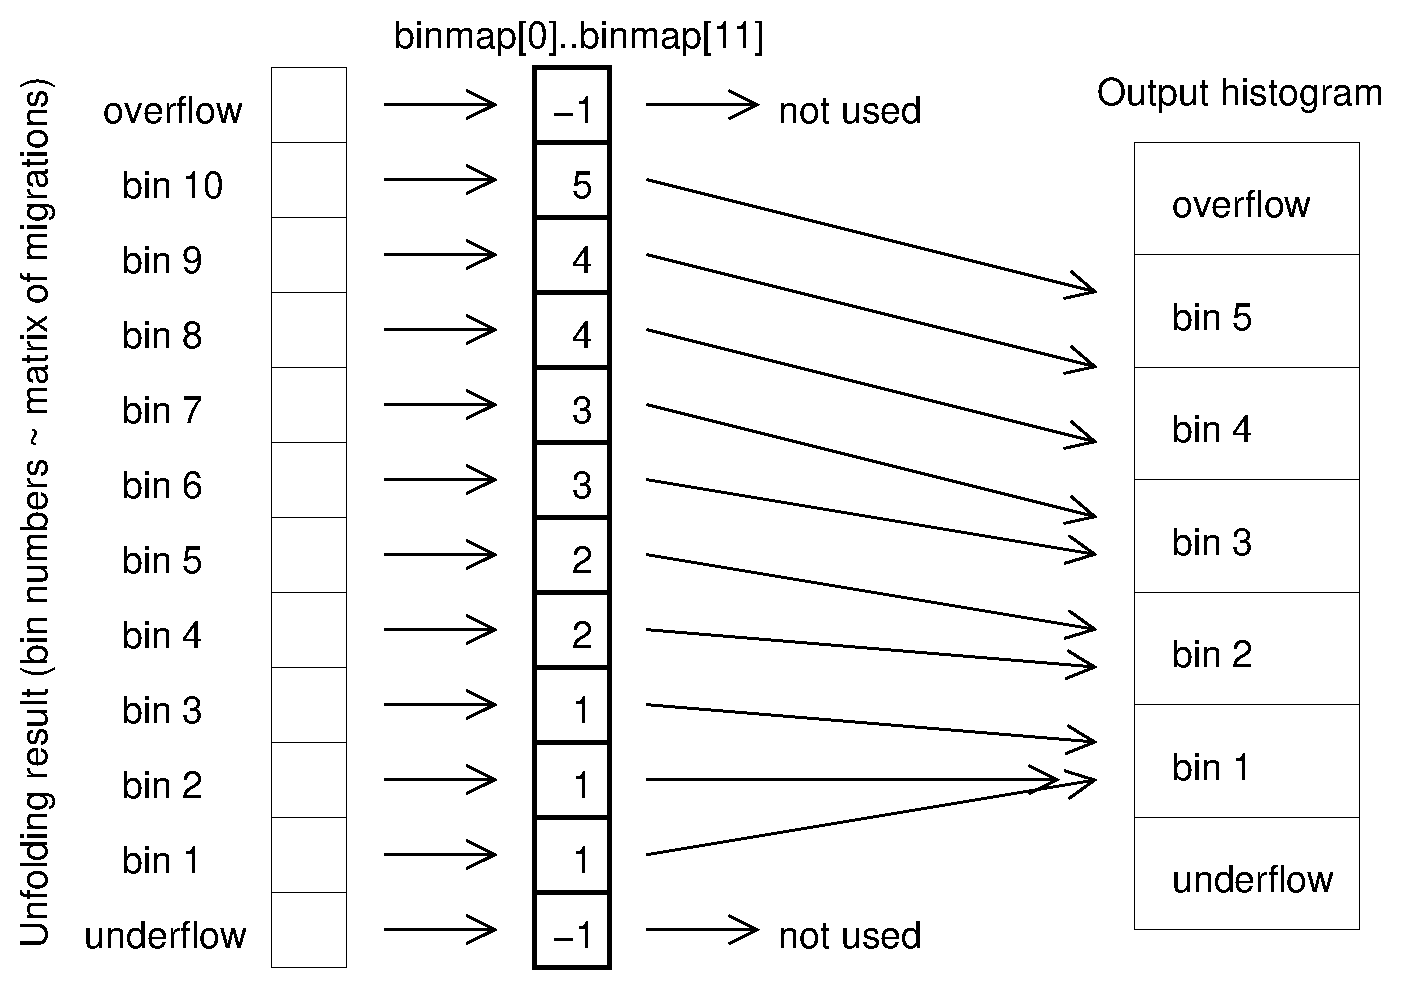
\includegraphics[width=0.7\figwidth]{tunfold_manual_fig1.eps}
\end{center}
\caption{\label{fig:binmap} For the classes {\tt TUnfold} and {\tt
  TunfoldSys}, the bin map defines which bins of the unfolding result
are stored in which histogram bin. In the example, 10 bins are mapped
to 5 bins.}
\end{figure}

\subsection{Binning schemes and TUnfoldDensity}

For the class {\tt TUnfoldDensity} the bins are structured in a
``binning scheme'' using the class {\tt TUnfoldBinning}.
For one-dimensional unfolding problems, the binning schemes are constructed
directly from the matrix of migrations. The user does not have to deal
with the class {\tt TUnfoldBinning}. For more complex problems,
involving multi-dimensional distributions, multiple channels or
unfolding of background normalisation factors,
the corresponding binning schemes have to be defined by the user.
The binning scheme information is used when setting
up the regularisation scheme. In addition, it is used to
create histograms having proper bin widths when extracting
data from the class {\tt TUnfoldDensity}. Furthermore, the binning
scheme provides functionality to find the proper bin numbers when
filling the histogram of migrations or the histogram of measurements.

\subsection{Unfolding one-dimensional distributions in TUnfoldDensity}

When unfolding one-dimensional distributions, it is most convenient to
book and fill the histogram of migrations using the bins as required for the
analysis. There is no need to define binning schemes.
The matrix of migrations is stored as a two-dimensional histogram, where on
one axis the truth bins are arranged. It is possible to have underflow
and overflow bins for the truth parameters. If these are present,
their content is also unfolded from the data.
On the other axis there is the reconstructed quantity, again with the
appropriate bins. Here, it is not possible to use the underflow and overflow
bins for measurements. Instead, these bins are used to count events
which originate from a specific truth bin but where the reconstructed quantity
is not available. An example is given in figure \ref{fig:unfold1dim}.
\begin{figure}
\begin{center}
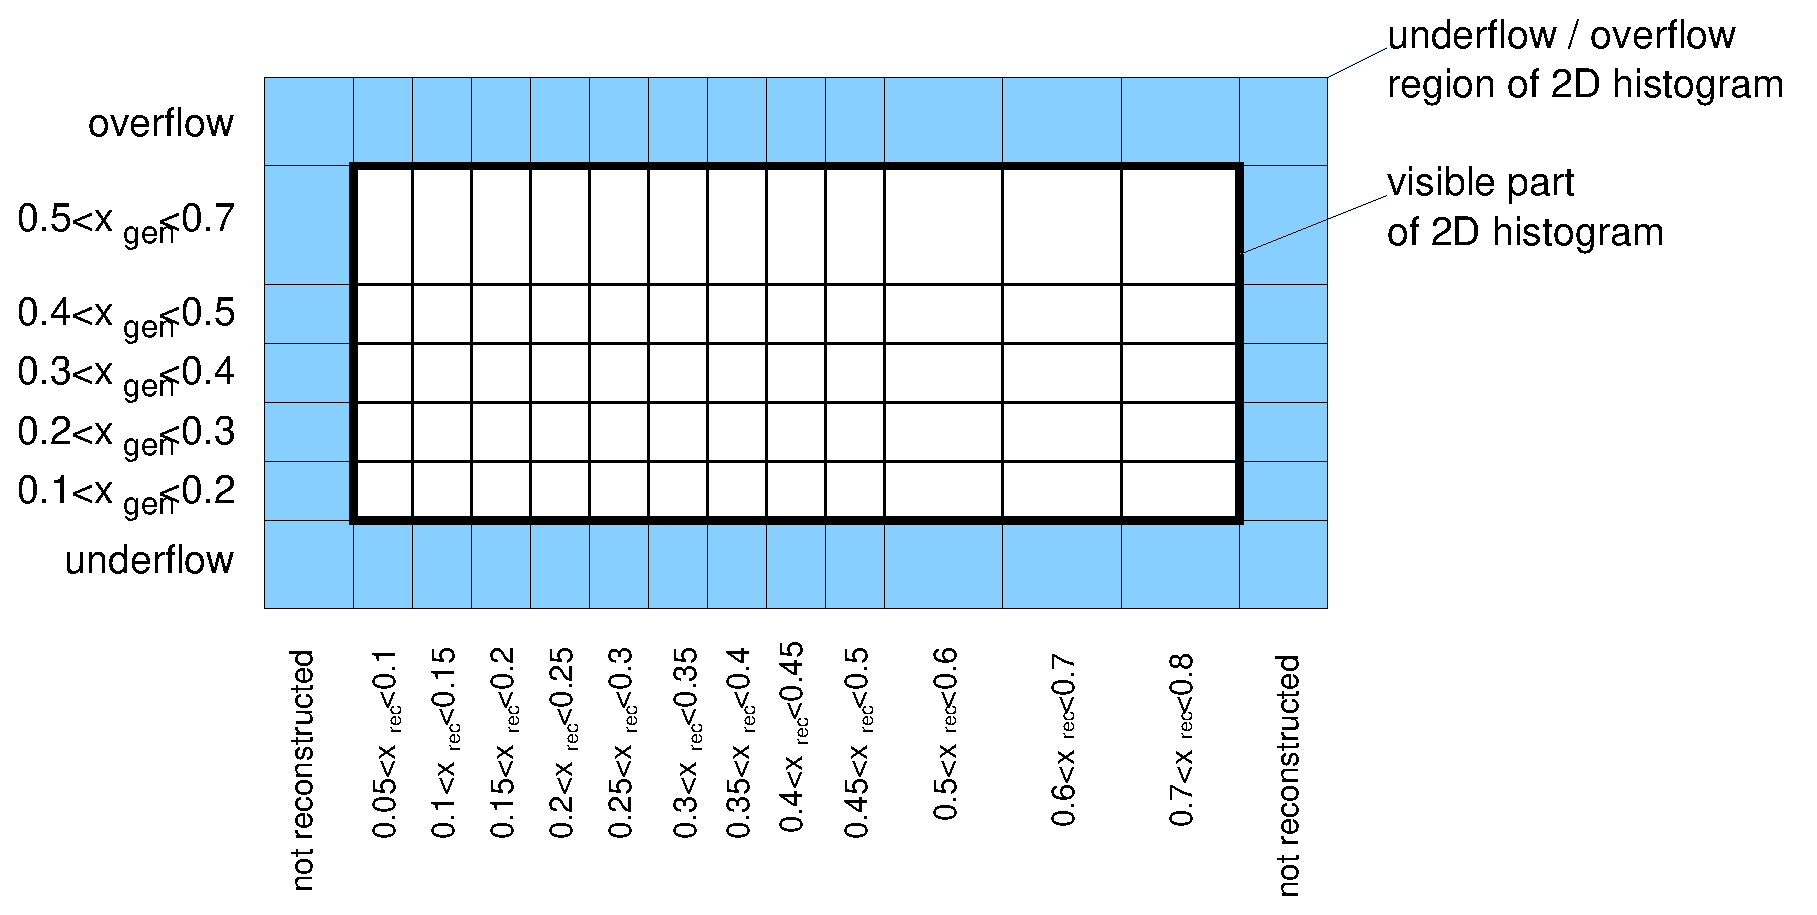
\includegraphics[width=0.7\figwidth]{tunfold_manual_fig2.eps}
\end{center}
\caption{\label{fig:unfold1dim} The matrix of migrations in the case of
  one-dimensional unfolding 
  is illustrated. The truth parameter $x_{\text{gen}}$ has five
  non-equidistant bins, 
  ranging from $0.1$ to $0.7$ plus underflow and overflow bins (seven bins in
  total).
  The reconstructed parameter $x_{\text{rec}}$ has twelve
  bins ranging from $0.05$ to $0.8$. The underflow and overflow bins in
  $x_{\text{rec}}$ are used to count the non-reconstructed events.
}
\end{figure}

\subsection{Complex binning schemes}

The class {\tt TUnfoldBinning} provides means to map bins originating from 
one or several multi-dimensional distributions on a single histogram
axis and back. The multi-dimensional distributions are arranged in a
tree structure.

For the truth parameters, the branches of the tree structure could
correspond to different decay channels, signal and background,
etc. Each branch then holds several bins, in most cases in the form of
a multi-dimensional histogram.
Similarly, for the reconstructed parameters, the branches of the
tree structure could correspond to different reconstructed channels
and various control distributions. 
So in general, there are two ``binning trees'', a tree of truth bins
and a tree of reconstructed bins.

When filling the histogram of migrations, the proper bin numbers both
in the tree of truth bins and in the tree of reconstructed bins have
to be determined. 
The bin number $i_{\text{gen}}$ on truth level is determined as
follows: first, the appropriate branch is determined, for example by
deciding on the event type (signal or background). The method {\tt
  FindNode()} may be used to locate a branch in the tree using its name.
Next, using the truth parameters, the bin number $i_{\text{gen}}$ is
calculated using the method {\tt GetGlobalBinNumber()} on the
branch. Below this is illustrated in a code fragment, assuming the
signal branch contains a three-dimensional histogram with the
variables {\tt xTrue}, {\tt yTrue}, {\tt zTrue}.

{\tt
\begin{verbatim}
  Int_t iGen;
  const TUnfoldBinning *signalBranch=generatorBinning->FindNode("signal");
  iGen=signalBranch->GetGlobalBinNumber(xTrue,yTrue,zTrue);
\end{verbatim}
}

The bin number $i_{\text{rec}}$ in the
tree of reconstructed bins is determined in a similar manner, for
example by deciding on the reconstructed channel and then using the
appropriate reconstructed quantities to calculate the bin number.
If the event was not reconstructed, the special bin number
$i_{\text{rec}}=0$ must be used.

Finally, the event weight $w_{\text{gen}}$ is filled in the
corresponding bin of the two-dimensional histogram of
migrations. Sometimes there is a secondary event weight
$w_{\text{rec}}$ to account for detector efficiency corrections. In
order to get the proper efficiency correction from the unfolding, the
event must be filled twice into the histogram of migrations: first,
the histogram of migration is filled at the position
$(i_{\text{gen}},i_{\text{rec}})$ using the weight
$w_{\text{gen}}\times w_{\text{rec}}$.
Next, the histogram of migration is filled again, this time at the
position $(i_{\text{gen}},0)$  using the event weight $w_{\text{gen}}\times(1-w_{\text{rec}})$.

For data, the procedure to determine the bin number $i_{\text{rec}}$
is applied for the reconstructed quantities only, and a
one-dimensional histogram is filled.

Setting up binning schemes with {\tt TUnfoldBinning} is illustrated in
the example macro {\tt testUnfold5b.C}. How to use the binning scheme to fill
histograms is illustrated in {\tt testUnfold5c.C}.
Unfolding and extracting distributions using the binning scheme is
illustrated in {\tt testUnfold5d.C}.

\subsection{XML interface to binning schemes}

An XML interface is provided for the binning schemes. The DTD
definition is repeated here. There is a method {\tt
  TUnfoldBinningXML::WriteDTD()} which saves the DTD to a file.
{\tt
\begin{verbatim}
<!-- TUnfold Version V17.3 -->
<!ELEMENT TUnfoldBinning (BinningNode)+ >
<!ELEMENT BinningNode (BinningNode+|(Binfactorlist?,Axis)|Bins) >
<!ATTLIST BinningNode name ID #REQUIRED firstbin CDATA "-1"
    factor CDATA "1.">
<!ELEMENT Axis ((Bin+,Axis?)|(Axis)) >
<!ATTLIST Axis name CDATA #REQUIRED lowEdge CDATA #REQUIRED>
<!ELEMENT Binfactorlist (#PCDATA)>
<!ATTLIST Binfactorlist length CDATA #REQUIRED>
<!ELEMENT Bin EMPTY>
<!ATTLIST Bin width CDATA #REQUIRED location CDATA #IMPLIED
    center CDATA #IMPLIED repeat CDATA #IMPLIED>
<!ELEMENT Bins (BinLabel)* >
<!ATTLIST Bins nbin CDATA #REQUIRED>
<!ELEMENT BinLabel EMPTY>
<!ATTLIST BinLabel index CDATA #REQUIRED name CDATA #REQUIRED>
\end{verbatim}
}
There are methods {\tt ExportXML} and {\tt ImportXML} to
write or read binning trees in XML format. One XML file may contain
several binning schemes. 

It is probably best to study the example macros {\tt testUnfold5a.C}--{\tt testUnfold5d.C} to find out how the XML interface works. In 
the example {\tt testUnfold5a.C}, pseudo events are written to root
files ``testUnfold5\_data.root'', ``testUnfold5\_signal.root'', ``testUnfold5\_background.root''. In {\tt testUnfold5b.C}, binning schemes are set up and then
stored as XML in a file named ``testUnfold5binning.xml''.
In {\tt testUnfold5c.C} the XML file is read and the binning schemes
are used when looping over the data, signal and background
events. Histograms required for the unfolding are filled. 
The histograms and the binning schemes are then stored in another root
file ``testUnfold5\_histograms.root''. Finally, the macro {\tt
  testUnfold5d.C} reads back that root file and runs the
unfolding. One could try to edit the XML file and run {\tt
  testUnfold5c.C} and {\tt testUnfold5d.C} repeatedly to see the
effects.

\section{Regularisation}

For unfolding, regularisation conditions are imposed. The
regularisation is given by the scalar product
$\left(\tau Lz,\tau Lz\right)$, where $z$ is the difference of the unfolding
result to a bias vector and $L$ is a matrix describing the
regularisation scheme. The parameter $\tau$ gives the strength of the
regularisation. The number of columns of $L$ is identical to
the number of unfolded bins. The number of rows reflects the number of
regularisation conditions, it may be different from the number of columns.

\subsection{Basic regularisation types}

Three basic types of regularisation are supported: {\tt kRegModeSize},
{\tt kRegModeDerivative}, {\tt kRegModeCurvature}. The type of
regularisation may be specified with the constructor of either of the
classes {\tt TUnfold}, {\tt TUnfoldSys}, {\tt TUnfoldDensity} as the
third argument. In that case, the given basic regularisation is
applied to all bins.

The simplest regularisation condition is given by {\tt kRegModeSize},
corresponding to the case where $L$ is the unity matrix.
The matrix $L$ is diagonal and does not mix different bins. The
regularisation is given by $\tau^2\sum z_i^2$.

For the condition {\tt kRegModeDerivative}, the matrix $L$
calculates differences $x_j-x_i$, thus approximating first
derivatives. In that case, the structure of the input bins matters,
because differences should be calculated between adjacent bins
only. For one-dimensional distributions this done by simply setting
$j=i+1$. For two-dimensional distributions, derivatives may be defined
along both dimensions and the relation is getting more complicated.
When using the classes {\tt TUnfoldDensity} and {\tt TUnfoldBinning},
the relation of the bins is known and appropriate regularisation schemes are
defined automatically.

For the condition {\tt kRegModeCurvature}, the matrix $L$ approximates
second derivatives $(x_k-x_j)-(x_j-x_i)$. Similar to the case of {\tt
  kRegModeDerivative} the corresponding matrix structure may get
rather complicated in case of multi-dimensional distributions, and is
most conveniently handled through the use of the classes {\tt
  TUnfoldDensity} and {\tt TUnfoldBinning}.

\subsection{Non-standard regularisation schemes}

Sometimes it is useful to set up non-standard regularisation
schemes. When using the class {\tt TUnfoldDensity} with user-defined
binning schemes, there is additional control over the regularisation
scheme. One may select modifications of the calculation of $L$ such
that the components of $z$ are normalized to the corresponding bin widths
prior to calculating the regularisation conditions. Furthermore, it is
possible to take into account the bin widths for the calculation of
the first or second derivatives. One may also set specific
normalisation factors or normalisation functions with the binning
scheme and use those to modify the normalisation of $z$ in the
calculation of the regularisation. 

For binning schemes based on trees with several branches it is possible
to restrict the regularisation to one of the branches or to set up
dedicated regularisation schemes for each of the branches (method {\tt
RegularizeDistribution()}).
For multi-dimensional distributions it is possible to exclude
underflow or overflow bins or to exclude derivatives calculated along
specific axes from the regularisation. Ultimatelty, it is also
possible to define arbitrary regularisation conditions by adding
single rows to the matrix $L$ (method {\tt AddRegularisationCondition()}).

\section{Determination of \protect\boldmath{$\tau$}}

One of the frequent questions related to the regularized unfolding method
implemented in the TUnfold package is the choice of the regularisation
parameter $\tau$. If $\tau$ is too small, there is no
regularisation. If $\tau$ is too large, the unfolding result is
biased strongly by the regularisation condition. In the TUnfold
package, two basic methods to determine the regularisation have been
implemented, the L-curve scan and the minimisation of
correlations.

\subsection{L-curve scan}

The L-Curve scan is available with the classes {\tt TUnfold}, {\tt
  TUnfoldSys} and {\tt TUnfoldDensity}. The method is named {\tt
  ScanLcurve}. It works as follows: the unfolding is repeated for a
number of points with different $\tau$, 
for example $n_p=30$. A parametric curve of two
variables $X(\tau)$ and $Y(\tau)$ is calculated.
The exact definition of these variables is given in 
\cite{Schmitt:2012kp}. The optimal chioce of $\tau$ is 
determined as the position having the largest curvature (``kink'') in
the $(X,Y)$ plane.
For scanning the L-curve, the following parameters may be set: number
of points $n_p$, minimum ($\tau_{\min{}}$) and maximum
($\tau_{\max{}}$) value of $\tau$ to scan. If
$\tau_{\min{}}=\tau_{\max{}}$, the interval is chosen
automatically. When running the scan, the following three curves are
produced: $X(\tau)$, $Y(\tau)$ and $Y(X)$.

The scan proceeds as follows: Given a $\tau$ interval to
scan, first the unfolding is performed for $\tau=\tau_{\min{}}$ and
$\tau=\tau_{\max{}}$. Intermediate points are then inserted such that
a most uniform population along the curve $X(\tau),Y(\tau)$ is
achieved. Given two or more
points $(X_i,Y_i)$, ordered in the corresponding $\tau_i$, a new point is
inserted into the interval which has the largest size $S^2=(X_{i+1}-X_i)^2+(Y_{i+1}-Y_i)^2$ until
$n_p-1$ points have been calculated.
The last point of the scan is inserted at the best choice of tau, determined
from the set of $n_p-1$ points.

\subsection{Minimisation of correlation coefficients or other quantities}

With the class {\tt TUnfoldDensity} another method of determining
$\tau$ is implemented. The method {\tt ScanTau()} repeats the unfolding $n_p$ times
for different choices of $\tau$. During that scan, the minimum of a
function $Z(\tau)$ is determined. The possible choices of the function
$Z$ are summarized in table \ref{tab:choiceOfZ}. They all depend on
the calculation of global correlation coefficients $\rho_i$, which is described in
\cite{Schmitt:2012kp}.
\begin{table}[ht]
\centering
\begin{tabular}{l|p{0.5\textwidth}}
Mode & definition of $Z$ \\
\hline
\hline
{\tt kEScanTauRhoAvg} & $Z=\frac{1}{n_{\text{bin}}}\sum_i \rho_i$
(average global correlation) \\
\hline
{\tt kEScanTauRhoMax} & $Z=\max_i \rho_i$
(maximum global correlation) \\
\hline
{\tt kEScanTauRhoAvgSys} & $Z=\frac{1}{n_{\text{bin}}}\sum_i \rho_{i,\text{sys}}$
(average global correlation, including systematic errors) \\
\hline
{\tt kEScanTauRhoMaxSys} &  $Z=\max_i \rho_{i,\text{sys}}$
(maximum global correlation, including systematic errors)\\
\hline
{\tt kEScanTauRhoSquareAvg} & $Z=\frac{1}{n_{\text{bin}}}\sum_i
(\rho_i)^2$
(average of squares of global correlation coefficients)\\
\hline
{\tt kEScanTauRhoSquareAvgSys} & 
$Z=\frac{1}{n_{\text{bin}}}\sum_i
(\rho_{i,\text{sys}})^2$ (average of squares of global correlation
coefficients including systematic errors)
\end{tabular}
\caption{\label{tab:choiceOfZ}Choices of the function $Z$ for
  implemented with the method {\tt ScanTau()}.}
\end{table}
When using the method {\tt ScanTau()}, the following parameters have
to be set: the number of points $n_p$, the  minimum and maximum value of $\tau$ to scan and
the mode (table \ref{tab:choiceOfZ}). If the minimum and maximum value
of $\tau$ agree, the scan range is determined automatically.
In addition one may change the
way the correlation coefficients $\rho_i$ are calculated. The
calculation may be restricted to one branch in the binning tree or may
use all branches. Within the distributions it is possible to exclude
underflow and overflow bins or to integrate over bins.
The scan returns four curves:
the curve $Z(\tau)$ and in addition the three curves also returned by
{\tt ScanLcurve()}.
For a given interval in $\tau$, $n_p-1$ points are inserted such that
large $\tau$ intervals are split into two.
Finally, using the set of $n_p-1$ points,
the position of the minimum is determined and the unfolding is
repeated at the position of the minimum.

The scan of correlation coefficients has the desired property that
correlations in the result are minimized. Ideally, the correlation
coefficients are small and can be neglected. However, this has to be
checked carefully.

A drawback of the method is that it often fails. In particular, this
method can not be used with the {\tt kRegModeSize}
regularisation condition. For the regularisation methods {\tt
  kRegModeDerivative} and {\tt kRegModeCurvature}, the method is
expected to work more reliably.

%\begin{appendix}
%\section{}
%\end{appendix}

\begin{flushleft}
\begin{thebibliography}{99}

%\cite{Schmitt:2012kp}
\bibitem{Schmitt:2012kp}
  S.~Schmitt,
  %``TUnfold: an algorithm for correcting migration effects in high energy physics,''
  JINST {\bf 7} (2012) T10003
  [arXiv:1205.6201].
  %%CITATION = ARXIV:1205.6201;%%

\bibitem{Brun:1997pa}
  R.~Brun and F.~Rademakers,
  %``ROOT: An object oriented data analysis framework,''
  Nucl.\ Instrum.\ Meth.\  A {\bf 389} (1997) 81.
  %%CITATION = NUIMA,A389,81;%%

\bibitem{tunfolddownload}
S.~Schmitt, TUnfold version \tunfoldversion, 
\url{http://www.desy.de/~sschmitt/tunfold.html}.

\end{thebibliography}
\end{flushleft}
\end{document}
